% =====================================================================
%  TECHNICAL REPORT -- Solute redistribution slider apps
%  Compile with:  tectonic TECHNICAL_REPORT.tex
%  or:            pdflatex TECHNICAL_REPORT.tex (twice)
% =====================================================================
\documentclass[11pt,a4paper]{article}

\usepackage[T1]{fontenc}
\usepackage[utf8]{inputenc}
\usepackage{lmodern}
\usepackage[margin=2.35cm,top=2.5cm,bottom=2.5cm]{geometry}
\usepackage{amsmath,amssymb}
\usepackage{graphicx}
\usepackage{booktabs,longtable,array}
\usepackage{xcolor}
\usepackage{hyperref}
\usepackage{xurl}
\usepackage{listings}
\usepackage{titlesec}
\usepackage{fancyhdr}
\usepackage{enumitem}
\usepackage{caption}
\usepackage{microtype}

% ---------------------------------------------------------------- colours
\definecolor{ink}{HTML}{0F172A}
\definecolor{teal}{HTML}{0F766E}
\definecolor{orange}{HTML}{C2410C}
\definecolor{blue}{HTML}{1D4ED8}
\definecolor{graytext}{HTML}{475569}
\definecolor{rulegray}{HTML}{CBD5E1}

\hypersetup{
  colorlinks=true,
  linkcolor=blue,
  urlcolor=teal,
  citecolor=teal,
  pdftitle={Solute Redistribution: Technical Report},
  pdfauthor={Prathamesh Deepak Ladhe},
  pdfsubject={MSE 670 Solidification -- interactive slider apps and MATLAB models}
}

\titleformat{\section}{\Large\bfseries\color{ink}}{\thesection}{0.7em}{}
\titleformat{\subsection}{\large\bfseries\color{ink}}{\thesubsection}{0.6em}{}
\titleformat{\subsubsection}{\normalsize\bfseries\color{graytext}}{\thesubsubsection}{0.5em}{}

\setlength{\parskip}{0.45em}
\setlength{\parindent}{0pt}
\setlength{\emergencystretch}{2em}

\pagestyle{fancy}
\fancyhf{}
\fancyhead[L]{\small\color{graytext}Solute Redistribution --- Technical Report}
\fancyhead[R]{\small\color{graytext}MSE 670}
\fancyfoot[C]{\small\thepage}
\renewcommand{\headrulewidth}{0.4pt}
\renewcommand{\headrule}{\hbox to\headwidth{\color{rulegray}\leaders\hrule height \headrulewidth\hfill}}

% ---------------------------------------------------------------- listings
% A small self-contained MATLAB language definition. Keeping it local means
% the report does not depend on listings' optional language-driver files.
\lstdefinelanguage{Matlab}{
  morekeywords={function,end,if,else,elseif,for,while,return,break,continue,
    switch,case,otherwise,try,catch,global,persistent,classdef,properties,
    methods,events,true,false,zeros,ones,linspace,size,numel,abs,exp,sqrt,
    max,min,plot,hold,grid,xlabel,ylabel,title,legend,figure,disp,fprintf,
    error,warning,assert,struct,arrayfun,cellfun},
  sensitive=true,
  morecomment=[l]\%,
  morestring=[b]'
}
\lstdefinestyle{matlab}{
  language=Matlab,
  basicstyle=\ttfamily\footnotesize,
  keywordstyle=\color{blue!70!black}\bfseries,
  commentstyle=\color{teal!80!black}\itshape,
  stringstyle=\color{orange!80!black},
  numbers=left,
  numberstyle=\tiny\color{graytext},
  numbersep=8pt,
  frame=single,
  rulecolor=\color{rulegray},
  backgroundcolor=\color{gray!4},
  breaklines=true,
  showstringspaces=false,
  columns=fullflexible,
  keepspaces=true,
  tabsize=4,
  captionpos=b,
  literate={*}{{\char42}}1
}
\lstset{style=matlab}

% ---------------------------------------------------------------- callout boxes
% Plain-LaTeX shaded callouts: no tcolorbox/pgf dependency, so the report
% compiles on a minimal TeX installation.
\newcommand{\calloutrule}[1]{\noindent{\color{#1}\rule{\linewidth}{0.8pt}}\par}
\newenvironment{callout}[2]{%
  \par\medskip\noindent
  \def\calloutcolor{#1}%
  \begin{minipage}{\linewidth}%
  \calloutrule{\calloutcolor}%
  \vspace{1pt}\par\noindent{\bfseries\small\color{\calloutcolor}#2}\par\vspace{2pt}%
  \small
}{%
  \par\vspace{2pt}\calloutrule{\calloutcolor}%
  \end{minipage}\par\medskip
}
\newenvironment{implnote}[1][]{\begin{callout}{blue!55!black}{#1}}{\end{callout}}
\newenvironment{provenance}[1][]{\begin{callout}{orange!70!black}{#1}}{\end{callout}}


\newcommand{\code}[1]{\texttt{\detokenize{#1}}}
\newcommand{\wtpct}{\,\mathrm{wt.\%}}

% =====================================================================
\begin{document}

% ---------------------------------------------------------------- title
\begin{titlepage}
\centering
\vspace*{1.2cm}

{\color{teal}\rule{\textwidth}{1.4pt}}\\[0.5cm]
{\Huge\bfseries\color{ink} Solute Redistribution in Solidification\par}
\vspace{0.35cm}
{\LARGE\color{graytext} Interactive Slider Applications and a\\[0.15cm]
Temperature-Coupled Microsegregation Model\par}
\vspace{0.5cm}
{\color{teal}\rule{\textwidth}{1.4pt}}\\[1.0cm]

{\Large\bfseries Technical Report\par}
\vspace{0.3cm}
{\large MSE 670 --- Solidification\par}
\vspace{1.4cm}

{\large
\begin{tabular}{@{}rl@{}}
\textbf{Author} & Prathamesh Deepak Ladhe\\[0.25cm]
\textbf{Course} & MSE 670, Solidification\\[0.25cm]
\textbf{Deliverables} & Browser app (\code{index.html}), MATLAB app (\code{fs_slider.m}),\\
 & five standalone model functions, documentation\\[0.25cm]
\textbf{Live demo} & \url{https://1clan.github.io/mse670-solute-redistribution/}\\[0.25cm]
\textbf{Repository} & \code{fs_slider_project}\\[0.25cm]
\textbf{Date} & \today\\
\end{tabular}\par}

\vfill

\begin{minipage}{0.86\textwidth}
\small\color{graytext}
\textbf{Scope.} This report documents the physical model, the numerical
implementation, the browser front end and the MATLAB front end. It states
every equation that is implemented, every default parameter with its
provenance, every simplifying assumption, and the tests used to verify that
the two front ends agree.
\end{minipage}

\vspace{1.0cm}
\end{titlepage}

\tableofcontents
\clearpage

% =====================================================================
\section{Introduction and scope}

\subsection{Purpose}

The project is a teaching tool for the solute-redistribution problem in
solidification. It answers a single question visually:

\begin{quote}
\emph{Given an Al--4.8\,wt.\%\,Cu alloy freezing from the liquid, how do the
solid and liquid compositions evolve as the solid fraction increases, and how
does that answer change when the assumptions about diffusion and mixing
change?}
\end{quote}

Four classical limits are implemented side by side because each one removes a
different assumption:

\begin{enumerate}[leftmargin=1.4em,itemsep=0.15em]
  \item \textbf{Equilibrium (lever rule)} --- complete diffusion in both phases.
  \item \textbf{Scheil--Gulliver} --- no solid diffusion, perfectly mixed liquid.
  \item \textbf{No solid diffusion with limited liquid diffusion} --- a
        diffusion boundary layer builds ahead of a planar interface.
  \item \textbf{Clyne--Kurz} --- finite back diffusion in the solid with a
        mixed liquid, optionally with the Won--Thomas coarsening correction.
\end{enumerate}

The temperature slider adds a second axis of exploration. It moves the
equilibrium tie-line and, while coupling is enabled, rescales the partition
coefficient and the two diffusivities so that the concentration curves respond
to temperature.

\subsection{Deliverables}

\begin{table}[h]
\centering
\footnotesize
\begin{tabular}{@{}p{0.30\textwidth}p{0.62\textwidth}@{}}
\toprule
\textbf{File} & \textbf{Role}\\
\midrule
\code{index.html} & Self-contained browser app: layout, styling, four models,
SVG charts, animations, temperature coupling. No external dependencies.\\
\code{fs_slider.m} & MATLAB app (\code{uifigure}) reproducing the models,
controls, charts and animations.\\
\code{models/equilibrium_model.m} & Lever-rule composition, scalar or vector.\\
\code{models/scheil_model.m} & Scheil--Gulliver composition and average solid.\\
\code{models/limited_liquid_model.m} & Mass-conserving solid profile plus
liquid boundary layer.\\
\code{models/clyne_kurz_model.m} & Back-diffusion model with optional direct
$\beta$ override.\\
\code{models/won_thomas_model.m} & Coarsening-corrected Clyne--Kurz.\\
\code{README.md} & Full model documentation and control reference.\\
\code{SITE\_OVERVIEW.md} & Plain-language guide to the deployed site.\\
\code{report/TECHNICAL\_REPORT.tex} & This report (source).\\
\code{preview.png} & Screenshot used in the README and this report.\\
\bottomrule
\end{tabular}
\end{table}

\subsection{What is template and what is authored}
\label{sec:provenance}

Because the graphical scaffolding and the physics are easy to confuse in a
single-file app, the project separates them explicitly. The same separation is
repeated as banner comments inside \code{fs_slider.m} and is summarised below.

\begin{provenance}[Provenance of the code]
\begin{itemize}[leftmargin=1.2em,itemsep=0.2em]
  \item \textbf{UI template (adapted):} the \code{uifigure}/\code{uigridlayout}
        arrangement, the widget styling, the axes layout and the general
        slider-app skeleton follow the course's MATLAB slider template. They
        were restyled and extended with extra panels, but they contain no
        solidification physics.
  \item \textbf{Authored for this project:} all solute-redistribution
        equations, the four model implementations, the temperature-coupling
        fits and Arrhenius scalings, the mass-conserving finite-difference
        integration of the limited-liquid model, the chart data preparation,
        the animation logic, the browser implementation and all documentation.
  \item The browser app has no template: its HTML, CSS, JavaScript and SVG
        rendering were written for this project.
\end{itemize}
\end{provenance}

\subsection{How to read this report}

Section~\ref{sec:physics} derives every equation. Section~\ref{sec:browser}
describes the website; Section~\ref{sec:matlab} describes the MATLAB app and
the five standalone functions in plain language. Section~\ref{sec:verification}
lists the checks that were run. Section~\ref{sec:assumptions} collects the
assumptions and limits in one place, and Section~\ref{sec:run} is a quick-start
guide. The appendices contain the full source of all five model functions, a
function reference and a glossary.

A four-page condensed version for submission (assumptions, material data and
sources, equations, results, limitations) is in
\code{report/TECHNICAL\_SUMMARY.pdf}.

% =====================================================================
\section{Physical model and notation}
\label{sec:physics}

\subsection{The one-dimensional solidification problem}

A bar of nominal composition $C_0$ (wt.\% Cu in Al) is frozen from one end. At
any instant a fraction $f_s$ is solid and $1-f_s$ is liquid. The interface is
assumed planar and to advance normal to itself. Two relations are used
everywhere:

\begin{align}
  \text{local equilibrium at the interface:}\qquad & C_S^* = k\,C_L^*, \label{eq:partition}\\
  \text{solute conservation over the whole bar:}\qquad &
  f_s\,\overline{C_S} + (1-f_s)\,\overline{C_L} = C_0. \label{eq:balance}
\end{align}

Here $k$ is the partition coefficient, $C_S^*$ and $C_L^*$ are the interface
compositions, and bars denote averages over each phase. The models differ only
in how they close the relation between the interface value and the average ---
that is, in what they assume about diffusion.

\begin{table}[h]
\centering
\small
\begin{tabular}{@{}lll@{}}
\toprule
\textbf{Symbol} & \textbf{Meaning} & \textbf{Default (Al--4.8\,wt.\%\,Cu)}\\
\midrule
$C_0$ & nominal composition & $4.8$ wt.\%\\
$k$ & partition coefficient $C_S^*/C_L^*$ & $0.173$ at 648\,$^\circ$C\\
$f_s$ & solid fraction & slider, $0$--$1$\\
$T$ & interface temperature & $648\,^\circ$C\\
$T_m$ & melting point of pure Al & $660.3\,^\circ$C\\
$T_{eut}$ & eutectic / solidus temperature & $548\,^\circ$C\\
$D_S$ & solid diffusivity & $4.8\times10^{-15}$\,m$^2$/s\\
$D_L$ & liquid diffusivity & $2.4\times10^{-9}$\,m$^2$/s\\
$v$ & growth velocity & $20\,\mu$m/s\\
$t_f$ & local solidification time & $100$\,s\\
$\lambda_2$ & secondary dendrite-arm spacing & $20\,\mu$m\\
$\alpha_C$ & Won--Thomas coarsening constant & $0.10$\\
$L$ & characteristic length for $\delta/L$ & $1$\,mm\\
\bottomrule
\end{tabular}
\caption{Notation and the reference parameter set.}
\end{table}

\subsection{Equilibrium: the lever rule}
\label{sec:equilibrium}

Complete diffusion in both phases keeps each phase uniform, so the interface
values equal the averages. Substituting $C_S^*=kC_L^*$ into
Eq.~\eqref{eq:balance} with $C_S=C_S^*$ and $C_L=C_L^*$ gives
\begin{equation}
  f_s\,kC_L + (1-f_s)\,C_L = C_0
  \quad\Longrightarrow\quad
  C_L = \frac{C_0}{1-(1-k)f_s},
\end{equation}
and therefore
\begin{equation}
  \boxed{C_S = \frac{kC_0}{1-(1-k)f_s}},
  \qquad
  \boxed{C_L = \frac{C_0}{1-(1-k)f_s}}.
  \label{eq:lever}
\end{equation}
At $f_s=0$ this returns $C_S=kC_0$ and $C_L=C_0$; at $f_s=1$ both phases reach
$C_0$. This is the equilibrium reference limit. For $k<1$ the denominator
vanishes beyond $f_s=1$, so the model is only evaluated on $[0,1]$.

\subsection{Scheil--Gulliver: no solid diffusion, mixed liquid}

With $D_S=0$ the solid retains the composition it had when it formed, while the
liquid stays uniform. Considering an increment of solid $df_s$:
\begin{equation}
  (C_L-C_S)\,df_s = (1-f_s)\,dC_L
  \quad\Longrightarrow\quad
  \frac{dC_L}{C_L} = (k-1)\frac{df_s}{1-f_s}.
\end{equation}
Integrating from $(f_s,C_L)=(0,C_0)$:
\begin{equation}
  \boxed{C_L = C_0(1-f_s)^{k-1}},
  \qquad
  \boxed{C_S^* = kC_0(1-f_s)^{k-1}}.
  \label{eq:scheil}
\end{equation}
The average solid composition follows from Eq.~\eqref{eq:balance}:
\begin{equation}
  \overline{C_S} = \frac{C_0\left[1-(1-f_s)^k\right]}{f_s},
  \qquad
  \overline{C_S}\to kC_0 \ \text{as}\ f_s\to0.
  \label{eq:scheilavg}
\end{equation}
For $k<1$ both interface compositions diverge as $f_s\to1$; the app caps the
plotted range and flags the singularity rather than drawing a finite artefact.

\subsection{No solid diffusion with limited liquid diffusion}
\label{sec:limited}

This is the Tiller--Jackson--Rutter--Chalmers picture. There is no solid
diffusion and no convective mixing, so rejected solute can only spread by
diffusion in the liquid. Ahead of a planar interface moving at $v$, the steady
boundary layer is
\begin{equation}
  C_L(z) = C_0 + \left(C_L^*-C_0\right)e^{-z/\delta},
  \qquad
  C_L(0)=C_L^*=\frac{C_0}{k},
  \qquad
  \boxed{\frac{\delta}{L}=\frac{D_L}{vL}},
  \label{eq:boundary}
\end{equation}
where $z$ is measured ahead of the interface and $L=1$\,mm is the
characteristic length. At steady state the solid grows at $C_S=C_0$ and
$C_L^*=C_0/k$.

\paragraph{Initial and final transients.} A pure exponential is not sufficient
over the whole bar: the first solid is enriched relative to $kC_0$, and near
the end of the bar the boundary layer is squeezed against the mould wall, which
produces a final spike. The implementation therefore integrates the solid
profile directly from local equilibrium plus global solute conservation.

Let $x\in[0,f_s]$ be the solidified coordinate and $S(x)=C_S(x)/C_0$ the
normalised solid composition. Define the cumulative solute
\begin{equation}
  I(f_s)=\int_0^{f_s} S(x)\,dx .
\end{equation}
The solute still in the liquid, expressed as an equivalent solid fraction, is
$f_s-I(f_s)$. If the liquid boundary layer occupies the remaining length
$\ell=1-f_s$ and must absorb that excess uniformly, then
\begin{equation}
  \frac{C_L^*}{C_0}=1+\frac{f_s-I(f_s)}{\delta\left(1-e^{-\ell/\delta}\right)} .
  \label{eq:deficit}
\end{equation}
Local equilibrium then gives $S(f_s)=k\,C_L^*/C_0$. The code solves
Eqs.~\eqref{eq:deficit} and \eqref{eq:partition} by fixed-point iteration on a
uniform grid ($N=2200$ intervals in the browser, $N=1400$ in MATLAB) with the
trapezoidal rule for $I$:
\begin{equation}
  I_i = I_{i-1}+\tfrac12\left(S_{i-1}+S_i\right)\Delta x,
  \qquad
  S_i^{(m+1)} = k\left[1+\frac{x_i-I_i^{(m)}}{\delta\left(1-e^{-(1-x_i)/\delta}\right)}\right],
\end{equation}
with eight iterations per grid point and $S_0=k$. This reproduces the initial
transient, the $C_S=C_0$ plateau and the final spike in one mass-conserving
sweep. The interface values are obtained by interpolation at the requested
$f_s$; the liquid profile is then Eq.~\eqref{eq:boundary} with
$C_L^*=C_S^*/k$.

\paragraph{Why the fixed point converges.} The right-hand side depends on $S$
only through the running integral, and each grid step changes $I$ by
$O(\Delta x)$. The map is therefore a contraction for small $\Delta x$, and
eight sweeps reduce the residual to round-off for the grid sizes used here.
The solver also clamps $1-x$ to $10^{-9}$ so the exponential near the wall
cannot divide by zero.

\subsection{Clyne--Kurz: finite back diffusion}

The liquid is fully mixed, but the solid retains a finite amount of back
diffusion. The dimensionless Fourier number uses half the arm spacing as the
diffusion distance:
\begin{equation}
  \alpha=\frac{D_S t_f}{X^2}=\frac{4D_S t_f}{\lambda_2^2},
  \qquad X=\frac{\lambda_2}{2}.
\end{equation}
Clyne and Kurz replace the Brody--Flemings parameter by
\begin{equation}
  \boxed{\beta = 2\alpha\left(1-e^{-1/\alpha}\right)-e^{-1/(2\alpha)}},
  \label{eq:beta}
\end{equation}
which is bounded between $0$ and $1$. The liquid composition is the
generalised back-diffusion form
\begin{equation}
  \boxed{\frac{C_L}{C_0}=\left[1-(1-\beta k)f_s\right]^{\frac{k-1}{1-\beta k}}},
  \label{eq:ck}
\end{equation}
with $C_S^*=kC_L$ and
\begin{equation}
  \overline{C_S}=\frac{C_0-(1-f_s)C_L}{f_s}.
\end{equation}

Two limits connect the model to the others:
\begin{itemize}[leftmargin=1.4em,itemsep=0.1em]
  \item $\beta\to0$ recovers Scheil--Gulliver, Eq.~\eqref{eq:scheil}.
  \item $\beta\to1$ recovers the equilibrium lever rule, Eq.~\eqref{eq:lever}.
\end{itemize}
The implementation handles $k=1$ and $1-\beta k=0$ as special cases
(Eq.~\eqref{eq:ck} becomes $C_L=C_0e^{(1-k)f_s}$) so that no $0/0$ is ever
evaluated. A user may also supply $\beta$ directly as a sensitivity variable;
in that mode $\alpha$ only affects the reported diagnostics.

\subsection{Won--Thomas coarsening correction}

Won and Thomas approximate dendrite coarsening by replacing the Fourier number:
\begin{equation}
  \boxed{\alpha^{+}=2\left(\alpha+\alpha_C\right)},
  \qquad \alpha_C=0.10,
\end{equation}
and then evaluating Eq.~\eqref{eq:beta} with $\alpha^{+}$. The factor of two
extends the result to columnar dendrites and $\alpha_C$ accounts for the
smaller arm spacing present before coarsening is complete. This is an
approximate correction, not a full coarsening model, and the original paper's
empirical arm-spacing fits are steel-specific and are deliberately not applied.

\subsection{Temperature coupling}
\label{sec:temperature}

The notes assume constant $k$, $D_L$ and liquidus slope $m$. The interactive
temperature knob is an explicit extension: it couples $T$ to the material
parameters through standard Al--Cu phase-diagram data and Arrhenius diffusion,
so that moving the slider changes the concentration curves.

\paragraph{Liquidus and solidus fits.} Two quadratics pass through the
phase-diagram anchors
\begin{align}
  \text{liquidus: } &(0,660.3),\ (4.8,648),\ (33,548),\\
  \text{solidus: }  &(0,660.3),\ (0.8304,648),\ (5.65,548),
\end{align}
with the composition in wt.\% and the temperature in $^\circ$C:
\begin{align}
  T &= -0.0298060391\,C_L^2-2.41943101\,C_L+660.3, \label{eq:liqfit}\\
  T &= -1.05070285\,C_S^2-13.93963508\,C_S+660.3. \label{eq:sol}
\end{align}
For a given $T$ the physical root is
\begin{equation}
  C(T)=\frac{-b-\sqrt{b^2-4a(c-T)}}{2a},
  \qquad a<0,\ b<0,\ c=660.3,
\end{equation}
and $C=0$ when $T\ge c$ or the discriminant is negative. The partition
coefficient then follows from the phase-diagram ratio:
\begin{equation}
  \boxed{k(T)=\frac{C_S(T)}{C_L(T)}}, \qquad k(T)=k_{\text{ref}}\ \text{if } C_L<10^{-8}.
\end{equation}

\paragraph{Arrhenius diffusivities.} Both diffusivities are anchored at
$T_{\text{ref}}=648\,^\circ$C:
\begin{align}
  D_S(T) &= D_{S,\text{ref}}\exp\!\left[-\frac{Q_S}{R_g}
           \left(\frac{1}{T+273.15}-\frac{1}{T_{\text{ref}}+273.15}\right)\right],
  \label{eq:dsT}\\
  D_L(T) &= D_{L,\text{ref}}\exp\!\left[-\frac{Q_L}{R_g}
           \left(\frac{1}{T+273.15}-\frac{1}{T_{\text{ref}}+273.15}\right)\right],
  \label{eq:dlT}
\end{align}
with $D_{S,\text{ref}}=4.8\times10^{-15}$\,m$^2$/s,
$D_{L,\text{ref}}=2.4\times10^{-9}$\,m$^2$/s, $Q_S=130$\,kJ/mol,
$Q_L=30$\,kJ/mol and $R_g=8.314462618$\,J\,mol$^{-1}$K$^{-1}$.

\begin{figure}[h]
\centering
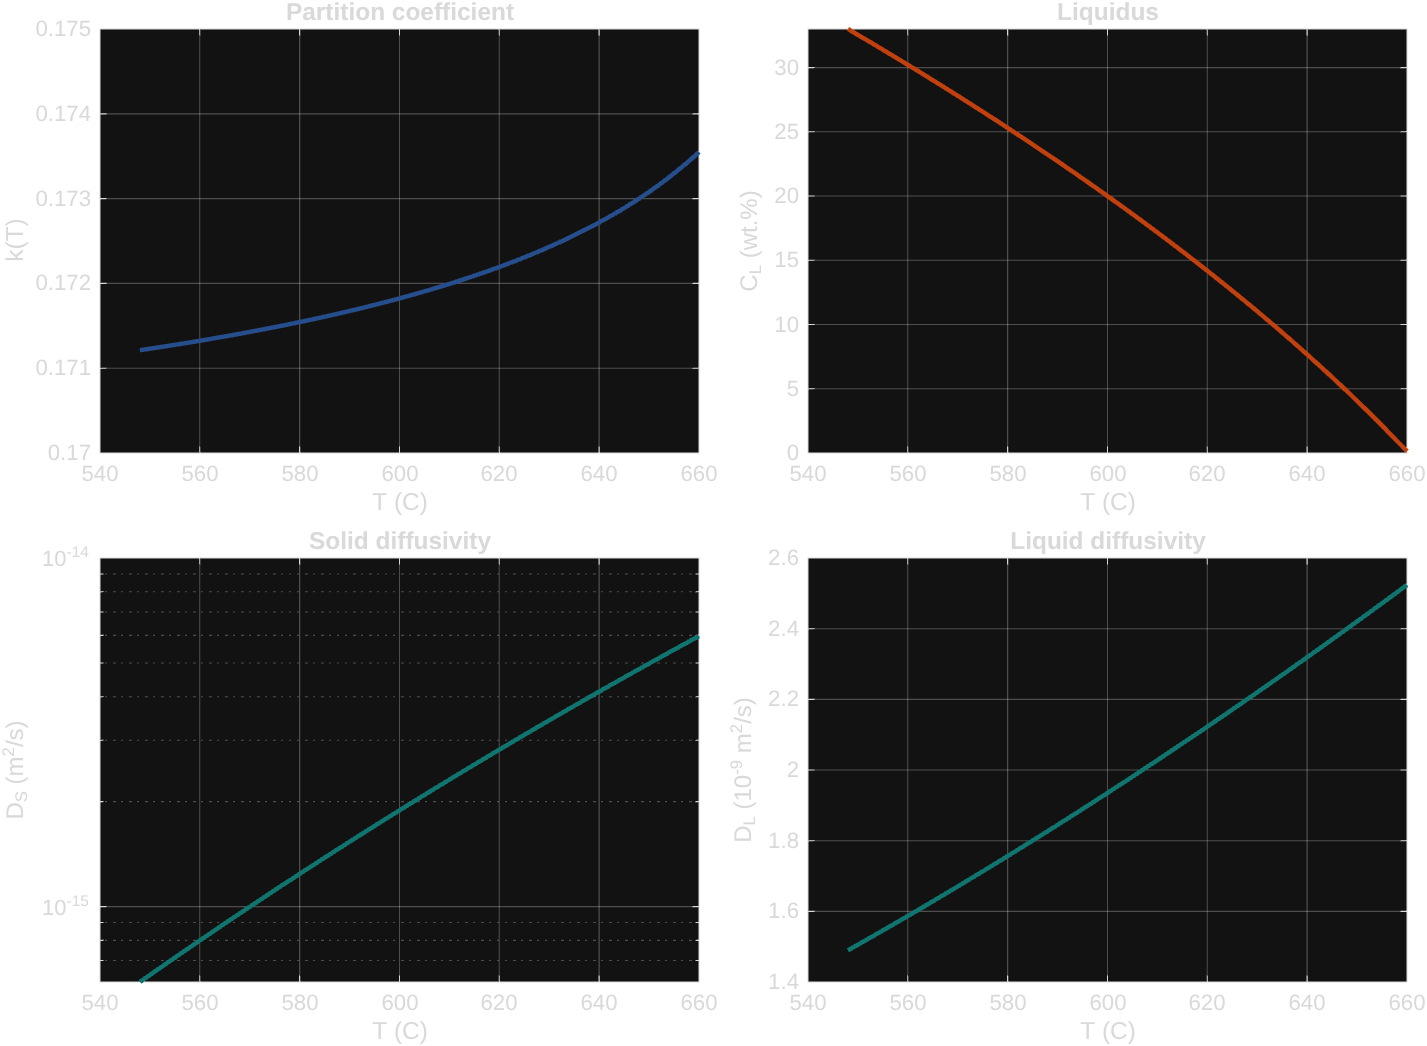
\includegraphics[width=\textwidth]{figures/fig_temperature.png}
\caption{Temperature coupling over the slider range. Top left: $k(T)$ is
almost flat for Al--Cu ($0.1712$ to $0.1735$). Top right: liquidus
composition from Eq.~\eqref{eq:liqfit}. Bottom row: Arrhenius
$D_S(T)$ and $D_L(T)$ from Eqs.~\eqref{eq:dsT}--\eqref{eq:dlT}.}
\label{fig:temperature}
\end{figure}

\paragraph{Consequences for the demo.} Figure~\ref{fig:temperature} makes an
important point explicit: $k(T)$ moves only by about $1.3\%$ across
$548$--$660\,^\circ$C. Because the normalised equilibrium and Scheil curves
depend only on $k$, they barely change with temperature. The visible
temperature effect is dominated by $D_S(T)$, which is about $7.9$ times smaller
at $548\,^\circ$C than at $648\,^\circ$C, and acts through $\alpha$ in
Clyne--Kurz and through $\delta/L$ in the limited-diffusion model.

\paragraph{The notes' spatial model.} Pages 7--9 of the handwritten notes go
further and combine the steady profile with a thermal gradient:
\begin{align}
  C_L(z) &= C_0\left[1+\frac{1-k}{k}e^{-Rz/D_L}\right],\\
  T_i &= T_m-\frac{mC_0}{k},\\
  T_L(z) &= T_i+mC_0\frac{1-k}{k}\left[1-e^{-Rz/D_L}\right],\\
  T(z) &= T_i+G_L z,\\
  \frac{G_L}{R} &\ge \frac{mC_0(1-k)}{kD_L}.
  \label{eq:supercooling}
\end{align}
This spatial model is \emph{not} what the temperature slider evaluates: it
requires a thermal gradient $G_L$ and a distance axis, neither of which is an
input to the current app. It is documented here because it is the notes'
temperature model and because Eq.~\eqref{eq:supercooling} is the natural next
extension (Section~\ref{sec:roadmap}). The interactive slider instead uses the
tie-line/fit route above, which is well posed for the available controls.

\subsection{Numerical edge cases}

\begin{table}[h]
\centering
\small
\begin{tabular}{@{}p{0.24\textwidth}p{0.66\textwidth}@{}}
\toprule
\textbf{Case} & \textbf{Implementation}\\
\midrule
$k=1$ & Clyne--Kurz returns $C_L=C_0$; Scheil and lever rule stay finite.\\
$1-\beta k=0$ & Eq.~\eqref{eq:ck} evaluated as $C_L=C_0e^{(1-k)f_s}$.\\
$\alpha\to0$ & $\beta\to0$ (Scheil limit); $\alpha\to\infty$ gives $\beta\to1$.\\
$f_s\to0$ & Averages evaluated analytically ($\overline{C_S}=kC_0$), not by $0/0$.\\
$f_s\to1$ & Singularities flagged; limited-liquid returns \code{Inf}, not a fake finite value.\\
$T\ge T_m$ & Fully liquid: tie-line shown as dashes/blank, $k$ held at $k_{\text{ref}}$ for the limiting curves.\\
$C_L<10^{-8}$ & $k(T)$ falls back to $k_{\text{ref}}$ instead of dividing by zero.\\
discriminant $<0$ & Fit root returns $0$ instead of a complex number.\\
$1-x\le0$ & Clamped to $10^{-9}$ inside the boundary-layer solver.\\
\bottomrule
\end{tabular}
\caption{Guarded cases in the JavaScript and MATLAB implementations.}
\end{table}

% =====================================================================
\section{The browser application}
\label{sec:browser}

\subsection{Architecture}

\code{index.html} is a single file with inline CSS and one JavaScript IIFE. It
has no frameworks, no build step, no CDN, no web fonts and no network requests.
It works from the filesystem (\code{file://}) and from GitHub Pages.

The script is organised in five layers:

\begin{enumerate}[leftmargin=1.4em,itemsep=0.15em]
  \item \textbf{Data and state.} An \code{ALLOY} constant holds the reference
        material; a single mutable \code{state} object holds every input
        ($f_s$, $T$, $k$, $C_0$, model, view, $v$, $D_L$, $D_S$, $t_f$,
        $\lambda_2$, $\alpha_C$, the two toggles and the direct $\beta$).
  \item \textbf{Model functions.} Pure functions of the state:
        \code{cs()}, \code{cl()}, \code{csAvg()}, \code{clAvg()},
        \code{ckCLNorm()}, \code{ckAvgNorm()}, \code{limitedSolidProfileNorm()},
        \code{limitedLiquidProfileNorm()}, plus the temperature helpers
        \code{liquidusC()}, \code{solidusC()}, \code{kAtT()},
        \code{dsAtT()}, \code{dlAtT()}.
  \item \textbf{Readout sync.} \code{syncTemperature()},
        \code{syncParameterSliders()}, \code{syncModelUI()},
        \code{updateParamHints()}.
  \item \textbf{Rendering.} \code{buildChart()} and
        \code{buildSpatialChart()} rebuild two SVG groups from scratch on every
        update using a small \code{svgEl()} helper.
  \item \textbf{Events.} Sliders, number fields, model/view buttons and play
        buttons call \code{setState(patch)}, which merges the patch and runs
        \code{update()}.
\end{enumerate}

The single entry point is \code{update()}: it syncs the derived properties and
labels, recomputes the compositions, redraws both charts and refreshes the
mass-balance check. Every interaction goes through it, so the readout and the
charts can never disagree.

\subsection{State and update flow}

\begin{center}
\small
\fbox{\parbox{0.94\textwidth}{
\centering
user input $\rightarrow$ \code{setState(patch)} $\rightarrow$
\code{Object.assign(state, patch)} $\rightarrow$ \code{update()} $\rightarrow$
\code{syncTemperature()} $\rightarrow$ \code{syncParameterSliders()} $\rightarrow$
model evaluation $\rightarrow$ \code{buildChart()} + \code{buildSpatialChart()}
}}
\end{center}

\code{syncTemperature()} is the only place that writes derived material
properties back into \code{state}. When \code{state.tempLinked} is true it sets
\code{state.k = kAtT(T)}, \code{state.ds = dsAtT(T)} and
\code{state.dl = dlAtT(T)}, and mirrors them into the number fields. When it is
false it only refreshes the readouts, so a manual $k$, $D_S$ or $D_L$ survives a
temperature change. The two $D$ fields are disabled while coupling is on,
because a value typed there would be overwritten on the next frame.

\subsection{Controls and override semantics}

\begin{table}[h]
\centering
\small
\begin{tabular}{@{}p{0.26\textwidth}p{0.64\textwidth}@{}}
\toprule
\textbf{Control} & \textbf{Behaviour}\\
\midrule
$f_s$ slider & $0$--$1$ in steps of $0.001$; the badge always shows three decimals.\\
$T$ slider & $548$--$700\,^\circ$C in steps of $1\,^\circ$C; the badge is a
fixed-width element (84\,px) showing an integer, so the layout cannot shift as
the value changes.\\
$k$ slider & logarithmic $0.01$--$100$ over $1000$ internal steps; the number
field is always editable.\\
$C_0$ slider & the same logarithmic mapping, default $4.8$ wt.\%.\\
Model buttons & four-way switch; each model has its own blurb and equation card.\\
View switch & \emph{Auto zoom} rescales the along-bar chart with $f_s$;
\emph{Fixed scale} freezes axes and grid.\\
Play buttons & one per parameter; see Section~\ref{sec:animation}.\\
Coupling box & \emph{Derive k, D\textsubscript{s} and D\textsubscript{L} from T},
checked by default.\\
\bottomrule
\end{tabular}
\caption{Browser controls.}
\end{table}

Three interactions count as a manual override of the temperature coupling:
dragging the $k$ slider, typing in the $k$ number field, and starting the $k$
animation. Each one clears the coupling flag and unchecks the box. Re-checking
the box re-anchors all three derived properties at the current temperature. The
$k$ label and the tie-line label switch between \code{k(T)} and \code{k} so the
readout always names the value the curves are actually using.

\subsection{Charts}

Both charts are hand-built SVG. The main chart uses a $860\times500$ viewBox
with margins $\{24,30,66,82\}$ (top, right, bottom, left). It plots normalised
composition $C/C_0$ against $f_s$:

\begin{itemize}[leftmargin=1.4em,itemsep=0.1em]
  \item solid curve: $C_S(f_s)/C_0$;
  \item liquid curve: $C_L(f_s)/C_0$ (dashed except for the limited model,
        where the boundary-layer profile is drawn);
  \item for Clyne--Kurz, an additional average-solid curve;
  \item horizontal dashed tie-line references at $\pm 4\%$ of the selected
        solute fraction, labelled $C_L^*$ and $C_S^*$;
  \item a vertical interface marker with a solid--liquid connector;
  \item a shaded band for the current solid fraction.
\end{itemize}

The along-bar chart uses a $860\times320$ viewBox with a 30\,px bar above the
plot area. Its $x$ axis is position $x/L\in[0,1]$, tinted teal behind the solid
and amber ahead of the interface. The solid profile is model-dependent:
Scheil shows $k(1-x)^{k-1}$, the limited model shows the integrated profile, and
Clyne--Kurz shows the back-diffused average as a homogenised solid. The liquid
side shows either a flat composition or the decaying boundary layer.

Axes are recomputed on every draw. The normalised $y$ limit is the maximum of
the current curve values times a 6--12\,\% headroom, capped at 25 so that the
Scheil singularity cannot make the plot unreadable. In fixed-scale mode the
limit is the model-wide value, which keeps the grid identical while $f_s$
moves. Ticks come from a \code{ticksFor()} helper that chooses a round interval
for roughly six ticks.

\subsection{Animation}
\label{sec:animation}

Each play button sweeps its parameter from one end of its range to the other
and back. The animation is driven by \code{requestAnimationFrame} at a rate of
$0.18$ of the full range per second, with the frame step capped at 50\,ms so a
background tab cannot jump. Only one animation runs at a time; starting another
stops the previous one. Any manual slider or number-field edit stops the
animation. The temperature animation snaps to whole degrees and the $k$/$C_0$
animations use the same logarithmic mapping as their sliders, so the animation
path matches the slider path exactly. \code{prefers-reduced-motion} disables the
CSS transitions used for the badge and panel fades.

\subsection{Responsive layout and accessibility}

The page is a two-column layout (controls $+$ readout on the left, charts on
the right) above 900\,px. Below 900\,px it becomes a single column with the
chart first; below 560\,px the stat boxes stack. Every input has an
\code{aria-label}, each chart has a \code{<title>} and \code{<desc>}, model and
view buttons are \code{role="group"} with \code{aria-pressed}, and the play
buttons announce \emph{Animate}/\emph{Pause}. Colours were checked for
contrast on the light background. No information is carried by colour alone:
solid and liquid are distinguished by line style and labels as well.

\subsection{Performance}

The limited-liquid model is the only expensive one. Its solid-profile sweep is
cached on the key \code{k|delta}, so dragging $f_s$ or $T$ without changing
either parameter reuses the grid. The chart is rebuilt as a small number of
SVG nodes on each update, which is cheap at this size. All model functions are
pure and allocation-light; there is no global DOM query inside the render loop
(the elements are cached once in an \code{els} map).

\begin{figure}[h]
\centering
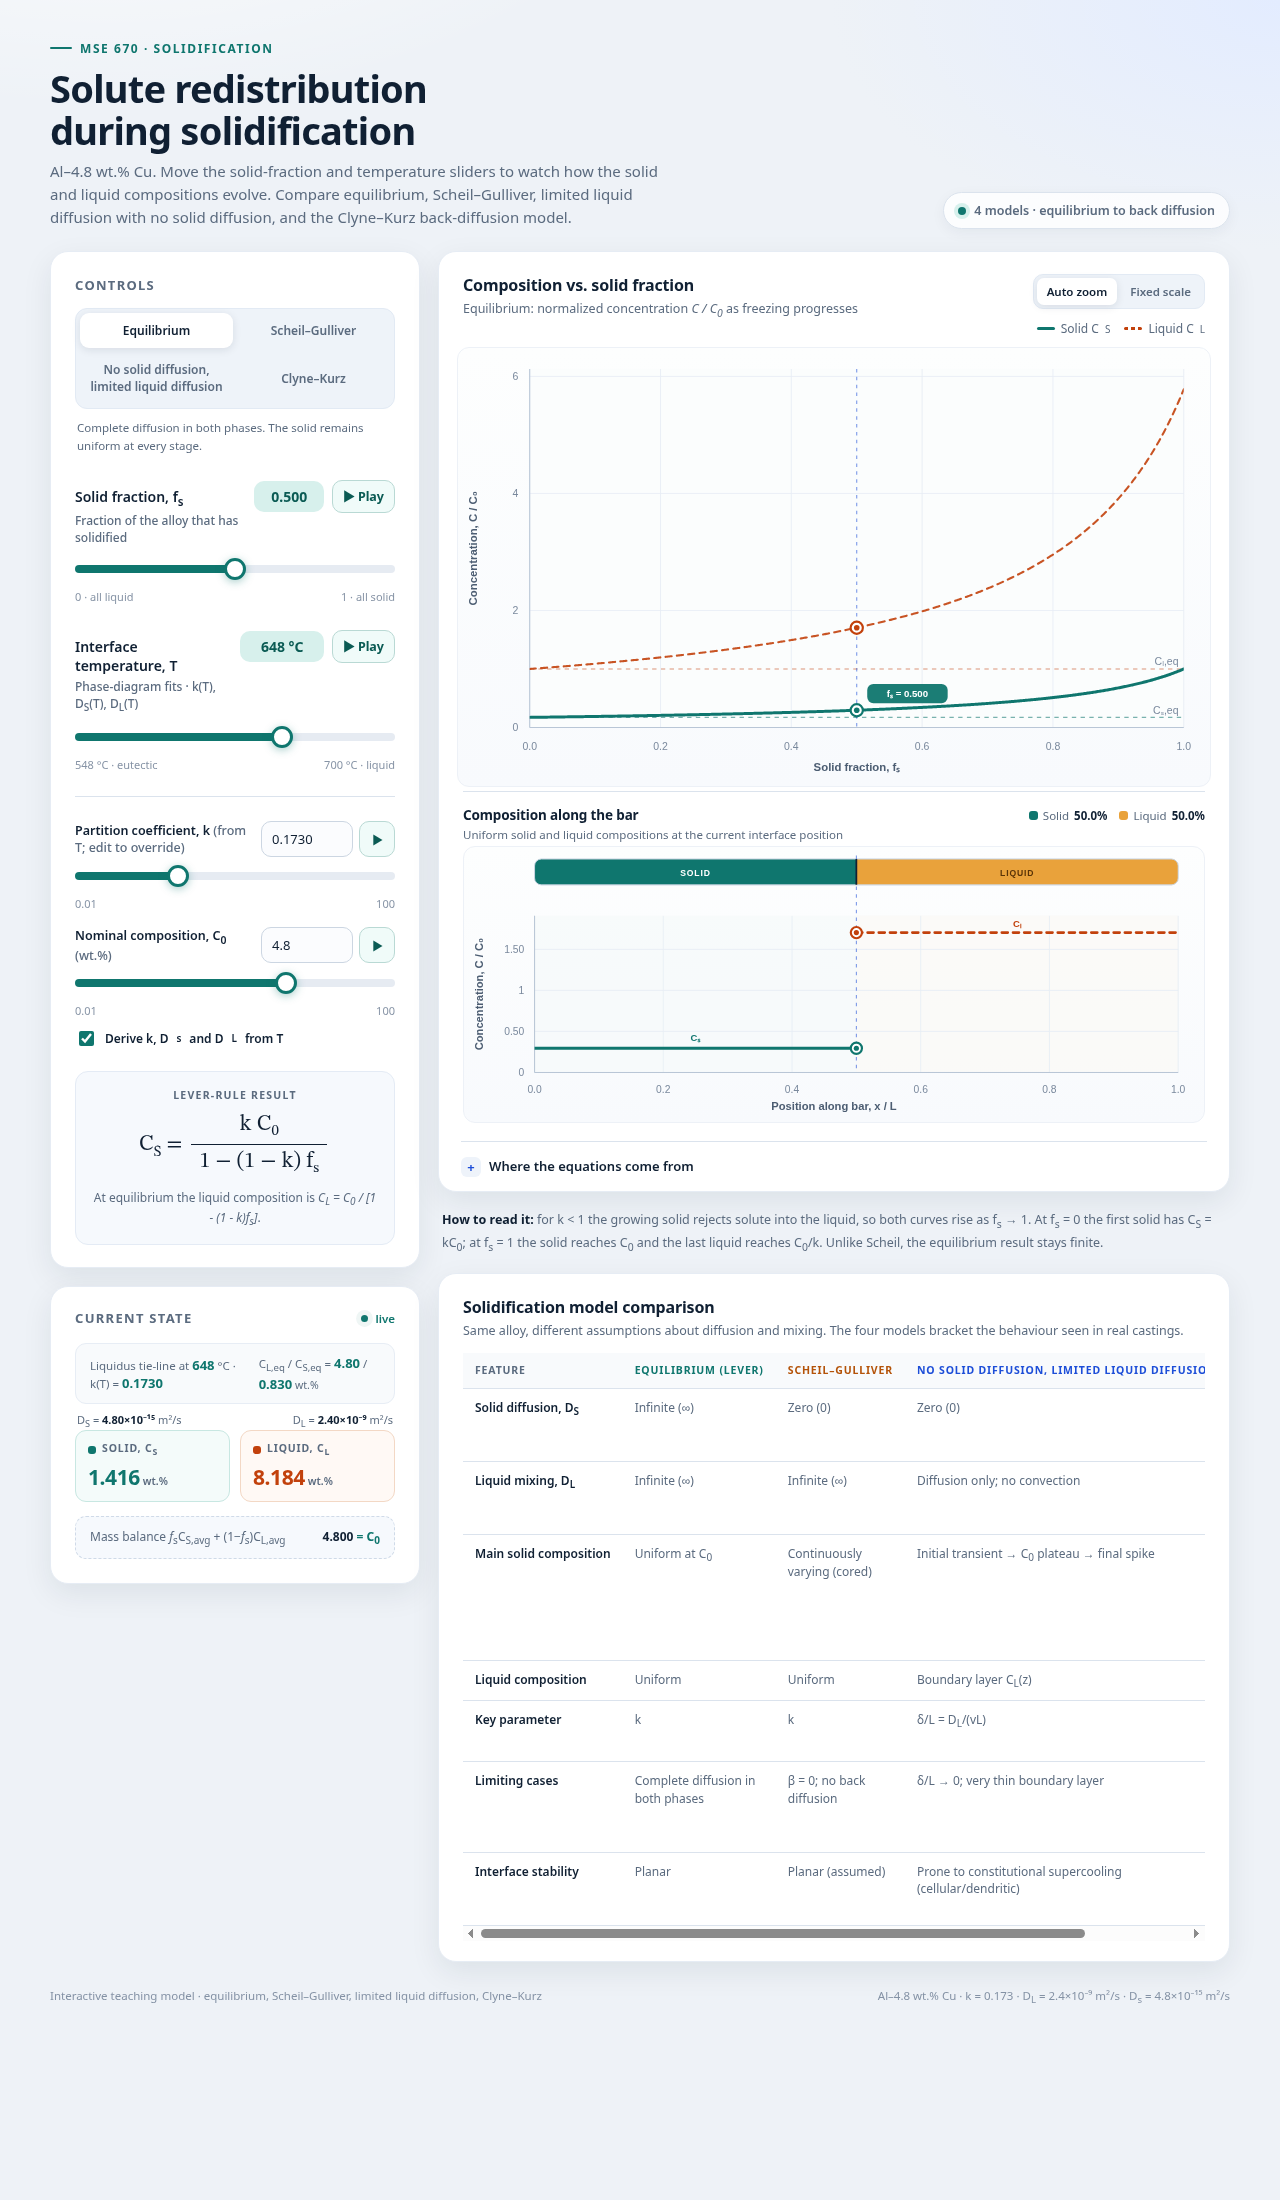
\includegraphics[width=\textwidth,height=0.80\textheight,keepaspectratio]{preview.png}
\caption{The browser app at the default state: controls and readout on the
left, composition chart and along-bar chart on the right.}
\label{fig:app}
\end{figure}

% =====================================================================
\section{The MATLAB application}
\label{sec:matlab}

\subsection{Requirements and how to run}

\begin{verbatim}
% Put the project folder on the path, then:
addpath('models');
fs_slider
\end{verbatim}

The app requires MATLAB R2020a or newer (\code{uifigure}, \code{uislider},
\code{uidropdown}, \code{uigridlayout}). It uses base MATLAB only: no
toolboxes, no external files, no network. It is self-contained in
\code{fs\_slider.m}; the \code{models/} functions are optional stand-alone
versions of the same equations and are linked from the documentation.

\subsection{Architecture: one function, nested callbacks}

\code{fs\_slider.m} is a single top-level function with no return value. All
widgets, state variables and helper functions live in its workspace; the
callbacks are \emph{nested functions}, so they read and write those variables
directly. This is the simplest possible MATLAB app architecture and is the main
reason the file reads linearly from top to bottom:

\begin{enumerate}[leftmargin=1.4em,itemsep=0.15em]
  \item \textbf{Parameters} (lines 46--72): material constants and defaults.
  \item \textbf{Part I --- UI template} (from \code{\%\% UI}): figure, grid
        layouts, widgets, styling, axes and plot objects. This is the adapted
        course template.
  \item \textbf{Part II --- authored logic}: callbacks, animation, temperature
        coupling, model equations, plotting and the update cycle.
\end{enumerate}

There is one shared clock for animation (\code{animTimer}, a MATLAB
\code{timer} at 20\,fps) and one entry point for refreshes:
\code{updateDisplay()}. Every callback ends by calling it, so the MATLAB app
has the same single-source-of-truth property as the browser app.

\subsection{The UI template part}

The figure is a $1180\times1000$ \code{uifigure} with a three-row
\code{uigridlayout}: header, controls/charts, and a status strip. The control
column is a 15-row $\times$ 3-column grid that stores one logical control per
row, so the vertical order of the interface is visible at a glance in the
\code{RowHeight} vector. Rows are shown or hidden by setting their height to
zero in \code{updatePanelLayout()}; this is how the model-specific parameter
panels change without rebuilding the figure.

\begin{table}[h]
\centering
\small
\begin{tabular}{@{}cl@{}}
\toprule
\textbf{Row} & \textbf{Control}\\
\midrule
1 & model dropdown\\
2 & temperature slider ($T$)\\
3--4 & tie-line label\\
5 & \emph{Derive k, D\textsubscript{s} and D\textsubscript{L} from T} checkbox\\
6 & solid-fraction slider ($f_s$)\\
7--8 & $k$ slider, number field and play button\\
9--10 & $C_0$ slider, number field and play button\\
11 & model-specific panel (limited liquid or Clyne--Kurz)\\
12--15 & status strip and footer labels\\
\bottomrule
\end{tabular}
\caption{Control-grid row map in \code{fs\_slider.m}.}
\end{table}

The two axes are created once and reused; \code{updateDisplay()} clears only
their children. The main axes shows composition versus $f_s$; the second axes
shows the along-bar profile and is re-titled with the current solid fraction.
Line objects for the curves, the tie-lines and the interface marker are
created once and their \code{XData}/\code{YData} are updated, which is the
recommended MATLAB pattern and avoids flicker.

\subsection{Callbacks and the update cycle}

\begin{center}
\small
\fbox{\parbox{0.94\textwidth}{
\centering
widget callback $\rightarrow$ \code{stopAnim()} $\rightarrow$
(optional override / rounding) $\rightarrow$ \code{updateDisplay()} $\rightarrow$
\code{syncTemperature()} $\rightarrow$ model evaluation $\rightarrow$
axes + readout
}}
\end{center}

\code{updateDisplay(fsRequested)} is the workhorse. It
refreshes the derived properties, evaluates the selected model, computes the
averages and the mass balance, builds the two plots and writes the readout
text. \code{syncTemperature()} writes derived $k$, $D_S$ and $D_L$ into the
numeric fields while coupling is on and disables the two diffusivity fields;
it leaves $k$ editable because typing there is the intended override gesture.

\subsection{Animation}

The four triangular buttons toggle a timer-driven sweep. \code{toggleAnim()}
records the target and the current normalised position, sets the direction, and
starts \code{animTimer} if it is not already running. \code{animStep()} advances
the position by $0.05\times0.18$ per tick, reflects it at the ends, and calls
the same setters a user would. Starting a $k$ animation clears the coupling
checkbox, matching the browser behaviour. \code{stopAnim()} deletes nothing: it
stops the timer and clears the target, so the timer object is reused. The
figure's \code{CloseRequestFcn} stops and deletes the timer before deleting the
figure, which prevents orphaned timers from keeping MATLAB busy.

\subsection{Plotting and panels}

The MATLAB plots are deliberately simpler than the browser SVG but follow the
same data pipeline: normalised composition, model-specific solid and liquid
curves, two dashed tie-line references, an interface marker and a shaded
solid-fraction band. The along-bar axes draws the solid profile on
$x/L\in[0,1]$ and the liquid boundary layer ahead of the interface. The view
dropdown switches between auto and fixed limits exactly as in the browser.

Parameter panels are toggled by row height, not by visibility alone, because a
zero-height row collapses cleanly in \code{uigridlayout}. The limited-liquid
panel shows $v$, $D_L$ and the derived $\delta/L$; the Clyne--Kurz panel shows
$D_s$, $t_f$, $\lambda_2$, $\alpha_C$, the direct-$\beta$ override and the
Won--Thomas checkbox. \code{updatePanelLayout()} is called on model changes and
from the update cycle, so the panel can never be out of step with the model.

\subsection{File-by-file guide}

\subsubsection{\code{fs\_slider.m} --- the app}

The header block states the author, the four model equations, the temperature
coupling, how to run, the MATLAB version requirement and the default material.
The file then defines parameters, builds the UI, and implements callbacks,
animation, coupling, models and plotting. Section banners mark the boundary
between the template and the authored logic. It has no dependencies beyond base
MATLAB and is the only file needed to run the app.

\subsubsection{\code{models/equilibrium\_model.m}}

Signature \code{[Cs, Cl, CsAvg, ClAvg] = equilibrium_model(k, c0, fs)}.
Evaluates Eq.~\eqref{eq:lever} vectorised over \code{fs}. \code{CsAvg} and
\code{ClAvg} are aliases of \code{Cs} and \code{Cl} because both phases are
uniform. Example: \code{equilibrium_model(0.173, 4.8, 0.5)} returns
$C_S=1.416$, $C_L=8.184$\,wt.\%.

\subsubsection{\code{models/scheil\_model.m}}

Signature \code{[Cs, Cl, CsAvg, ClAvg] = scheil_model(k, c0, fs)}.
Evaluates Eqs.~\eqref{eq:scheil}--\eqref{eq:scheilavg}. The average is computed
analytically and the $f_s\to0$ limit is handled separately rather than by
dividing by zero. \code{ClAvg} equals \code{Cl} because the liquid is mixed.

\subsubsection{\code{models/limited\_liquid\_model.m}}

Signature
\code{out = limited_liquid_model(k, c0, v, DL, fs, N, L)}.
Returns a struct with the solid grid, solid profile, $\delta$, interface
values, averages, the liquid grid and the boundary-layer profile. It performs
the fixed-point sweep described in Section~\ref{sec:limited} (default
$N=1400$, $L=1$\,mm) and returns \code{Inf} at the singular end point instead
of a finite artefact. Example:
\code{out = limited_liquid_model(0.173,4.8,20e-6,2.4e-9,0.5)} gives
$\delta/L=0.12$.

\subsubsection{\code{models/clyne\_kurz\_model.m}}

Signature
\code{out = clyne_kurz_model(k, c0, Ds, tf,}\\
\code{lambda2, fs, alphaC, useWT, betaOverride)}.
Returns $\alpha$, $\alpha_{\text{eff}}$, $\beta$, $C_L$, $C_S^*$,
$\overline{C_S}$ and $\overline{C_L}$. It implements
Eqs.~\eqref{eq:beta}--\eqref{eq:ck} with the special cases $k=1$ and
$1-\beta k=0$. When \code{betaOverride} is supplied, $\beta$ is clamped to
$[0,1]$ and used directly; $\alpha$ and the Won--Thomas flag then only affect
the diagnostics.

\subsubsection{\code{models/won\_thomas\_model.m}}

Signature
\code{out = won_thomas_model(k, c0, Ds, tf, lambda2, fs, alphaC)}.
A thin wrapper that calls \code{clyne\_kurz\_model(..., true)} and exposes
\code{alphaWT}. Default $\alpha_C=0.1$.

\begin{figure}[h]
\centering
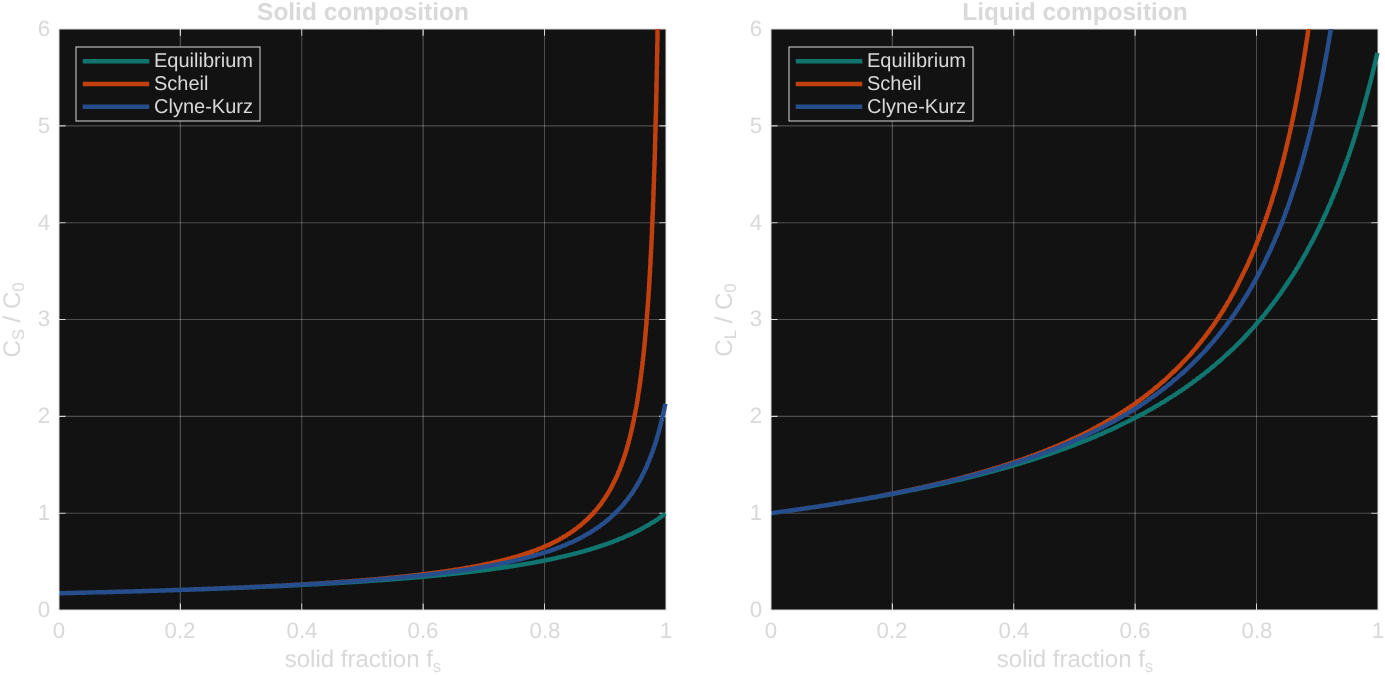
\includegraphics[width=\textwidth]{figures/fig_models.png}
\caption{Normalised solid and liquid compositions for three of the models at
the reference parameters ($k=0.173$, $C_0=4.8$\,wt.\%). The limited-liquid
model is spatial and is shown in Figure~\ref{fig:boundary}.}
\label{fig:models}
\end{figure}

\begin{figure}[h]
\centering
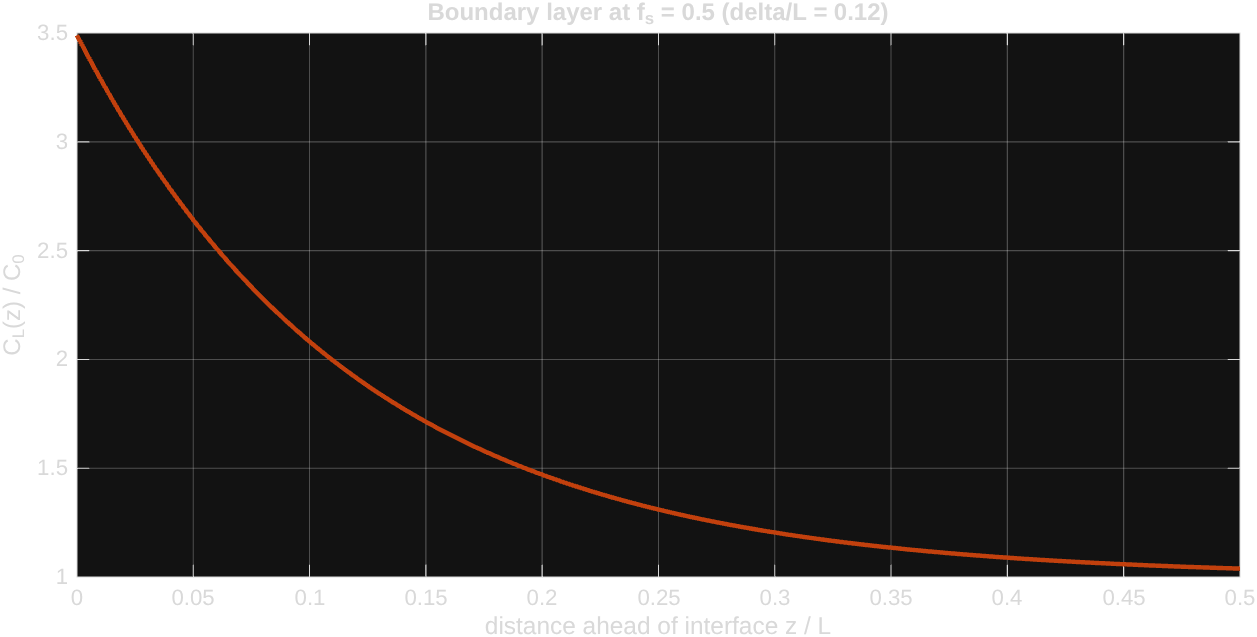
\includegraphics[width=0.82\textwidth]{figures/fig_boundary.png}
\caption{Liquid boundary layer ahead of the interface at $f_s=0.5$ from
Eq.~\eqref{eq:boundary}, $\delta/L=0.12$.}
\label{fig:boundary}
\end{figure}

\subsection{Template versus authored sections}

\begin{table}[h]
\centering
\small
\begin{tabular}{@{}p{0.34\textwidth}p{0.30\textwidth}p{0.26\textwidth}@{}}
\toprule
\textbf{Part of the file} & \textbf{Origin} & \textbf{Contains physics?}\\
\midrule
Parameter block & authored & defaults only\\
\code{\%\% UI} to end of widget creation & course template, adapted/restyled & no\\
\code{updatePanelLayout}, \code{syncParamSliders} & template pattern, extended & no\\
Callbacks and animation & authored & no (glue)\\
Temperature coupling & authored & yes\\
Model functions (\code{isScheil}, \code{ckCLNorm}, \code{limitedProfile}, \dots) & authored & yes\\
\code{updateDisplay} plotting data & authored & yes\\
Readout text & authored & descriptive\\
\bottomrule
\end{tabular}
\caption{Provenance map for \code{fs\_slider.m}. The file repeats this split as
banner comments so a reader can see it without this report.}
\end{table}

\subsection{Differences from the browser version}

The physics is identical; only the plumbing differs. The browser uses
$N=2200$ grid intervals in the limited model and MATLAB uses $N=1400$; both are
converged to plotting accuracy. The browser draws SVG by hand, MATLAB uses
\code{plot}/\code{fill}. The browser animates with
\code{requestAnimationFrame}, MATLAB with a 20\,fps \code{timer}. The browser
uses logarithmic sliders with 1000 internal steps, MATLAB uses its native
\code{uislider} with a position$\to$value mapping. The MATLAB $k$ and $C_0$
number fields use \code{ValueDisplayFormat} and the same override rules as the
website.

% =====================================================================
\section{Verification}
\label{sec:verification}

\subsection{What was checked}

\begin{table}[h]
\centering
\small
\begin{tabular}{@{}p{0.30\textwidth}p{0.44\textwidth}p{0.18\textwidth}@{}}
\toprule
\textbf{Check} & \textbf{Method} & \textbf{Result}\\
\midrule
JavaScript syntax & \code{node --check} on the extracted script & pass\\
Browser UI and coupling & headless Chrome (CDP), assertions on DOM values & pass\\
Browser models/views/animation & all four models, both views, all play buttons & pass\\
Temperature badge & integer text and constant 84\,px width at 548, 549, 640, 648, 700 & pass\\
Override semantics & drag/type/animate $k$ clears coupling; re-check re-anchors & pass\\
MATLAB static analysis & \code{checkcode('fs\_slider.m','-string')} & no messages\\
MATLAB app regression & scripted \code{uifigure} interaction & pass\\
Browser/MATLAB parity & $k(640)$, $D_S(640)$, $D_L(640)$, tie-line values & agree\\
Deployed page & fetch of the GitHub Pages URL & updated build served\\
\bottomrule
\end{tabular}
\caption{Verification performed before each release.}
\end{table}

\subsection{Reference values}

At the default state ($f_s=0.5$, $k=0.173$, $C_0=4.8$\,wt.\%) the equilibrium
model returns $C_S=1.416$ and $C_L=8.184$\,wt.\%. The temperature coupling
returns the values in Table~\ref{tab:tempcheck}.

\begin{table}[h]
\centering
\small
\begin{tabular}{@{}rrrrr@{}}
\toprule
$T$ ($^\circ$C) & $C_L$ (wt.\%) & $C_S$ (wt.\%) & $k(T)$ & $D_S$ (m$^2$/s)\\
\midrule
548 & 33.00 & 5.650 & 0.1712 & $6.07\times10^{-16}$\\
600 & 20.00 & 3.436 & 0.1718 & $1.89\times10^{-15}$\\
640 & 7.67  & 1.324 & 0.1727 & $4.14\times10^{-15}$\\
648 & 4.80  & 0.830 & 0.1730 & $4.80\times10^{-15}$\\
660 & 0.12  & 0.021 & 0.1735 & $5.97\times10^{-15}$\\
\bottomrule
\end{tabular}
\caption{Values reproduced by both front ends. $D_L$ moves from
$1.49\times10^{-9}$ at 548\,$^\circ$C to $2.96\times10^{-9}$ at 700\,$^\circ$C.}
\label{tab:tempcheck}
\end{table}

\subsection{How to reproduce the checks}

The test scripts are deliberately kept outside the repository so that the
deliverable stays small. They use only Node's built-in \code{assert} and the
Chrome DevTools Protocol, plus MATLAB's own \code{assert}:

\begin{verbatim}
# syntax
python3 -c "import re;print(re.findall(r'<script>(.*?)</script>',
  open('index.html').read(), re.S)[-1])" > /tmp/app.js
node --check /tmp/app.js

# MATLAB static analysis
matlab -batch "checkcode('fs_slider.m','-string')"
\end{verbatim}

The headless tests start Chrome with
\code{--headless=new --remote-debugging-port=9222}, open \code{index.html},
dispatch real \code{input} and \code{change} events, and assert on the DOM.
The MATLAB test builds the app, locates the widgets by type and limits, drives
the callbacks, and asserts on field values and labels.

% =====================================================================
\section{Assumptions and limitations}
\label{sec:assumptions}

\subsection*{Physical assumptions, common to all models}

\begin{enumerate}[leftmargin=1.4em,itemsep=0.18em]
  \item One-dimensional, planar interface advancing at constant velocity.
  \item Local equilibrium at the interface, $C_S^*=kC_L^*$. The models differ
        in the diffusion assumptions, not in the interface condition.
  \item Constant partition coefficient within a single model evaluation. The
        temperature coupling deliberately relaxes this as a sensitivity study.
  \item Constant densities and no convection, except where a model assumes the
        liquid is fully mixed.
  \item The terminal eutectic is not modelled. The eutectic composition
        ($\approx33$\,wt.\%) is used only as a phase-diagram anchor.
  \item Solute transport is described by Fick's law with a single diffusivity
        per phase.
\end{enumerate}

\subsection*{Model-specific assumptions}

\begin{itemize}[leftmargin=1.4em,itemsep=0.18em]
  \item \textbf{Equilibrium:} infinite diffusion in both phases; the result is
        an ideal reference limit, not a casting prediction.
  \item \textbf{Scheil:} zero solid diffusion and perfect liquid mixing. The
        interface composition diverges as $f_s\to1$ for $k<1$; the app caps
        the view and flags the singularity.
  \item \textbf{Limited liquid:} no solid diffusion, no liquid mixing. The
        boundary-layer form is the steady solution; the transient is captured
        by the mass-conserving sweep. Requires $\delta/L<1$ for a thin layer;
        the interface is assumed planar although it may be constitutionally
        supercooled.
  \item \textbf{Clyne--Kurz:} finite back diffusion, mixed liquid. It is an
        analytical approximation and does not resolve a spatial solid profile.
        The Won--Thomas correction is approximate and its empirical
        arm-spacing fits are steel-specific, so they are not used.
\end{itemize}

\subsection*{Temperature coupling}

\begin{itemize}[leftmargin=1.4em,itemsep=0.18em]
  \item The quadratic liquidus/solidus fits and the activation energies are
        standard Al--Cu approximations. They are an \emph{extension} beyond the
        notes, which assume constant $k$, $D_L$ and $m$.
  \item The fits are extrapolated across 548--700\,$^\circ$C. They should be
        used near the alloy composition, not as a full phase-diagram
        prediction.
  \item $k(T)$ is nearly flat for Al--Cu, so the equilibrium and Scheil
        \emph{normalized} curves barely respond to temperature; most of the
        visible effect is through $D_S(T)$ and $D_L(T)$.
  \item The notes' spatial model ($T_L(z)$, $G_L$, constitutional
        supercooling) is documented but not driven by the slider, because the
        app has no thermal-gradient or distance input.
\end{itemize}

\subsection*{Numerical assumptions}

The limited-liquid sweep uses a uniform grid and eight fixed-point iterations
per node; both are converged for plotting. The Scheil and Clyne--Kurz
singularities are capped or flagged. The browser caps the $y$ range at 25 so a
divergence cannot destroy the scale. All displayed values are rounded for
legibility; the underlying computation is double precision.

% =====================================================================
\section{Quick start}
\label{sec:run}

\subsection*{Browser}

\begin{verbatim}
cd fs_slider_project
python3 -m http.server 8000
# open http://localhost:8000
\end{verbatim}
or simply open \code{index.html} directly. The live copy is at
\url{https://1clan.github.io/mse670-solute-redistribution/}.

\subsection*{MATLAB app}

\begin{verbatim}
cd fs_slider_project
fs_slider
\end{verbatim}

\subsection*{Stand-alone model functions}

\begin{verbatim}
addpath('models');
[Cs, Cl] = equilibrium_model(0.173, 4.8, 0.5);
out = scheil_model(0.173, 4.8, linspace(0,1,50));
out = limited_liquid_model(0.173, 4.8, 20e-6, 2.4e-9, 0.5);
out = clyne_kurz_model(0.173, 4.8, 4.8e-15, 100, 20e-6, 0.5);
out = won_thomas_model(0.173, 4.8, 4.8e-15, 100, 20e-6, 0.5);
\end{verbatim}

\subsection*{This report}

\begin{verbatim}
cd report
tectonic TECHNICAL_REPORT.tex
# produces TECHNICAL_REPORT.pdf
\end{verbatim}

% =====================================================================
\section{Roadmap}
\label{sec:roadmap}

The most natural extension is the notes' spatial temperature model. It needs
only two additions: a thermal-gradient input $G_L$ and a temperature axis.
With $T_i=T_m-mC_0/k$ and the profile of Eq.~\eqref{eq:supercooling}, the app
could plot $T_L(z)$ and $T(z)=T_i+G_Lz$, shade the region where $T<T_L$, and
show the constitutional-supercooling criterion
$G_L/R\ge mC_0(1-k)/(kD_L)$ as a pass/fail badge. That would make temperature
reshape the \emph{profile}, not just the tie-line, while keeping the notes'
constant-property assumptions inside the spatial model.

Other extensions, in rough order of value: a CALPHAD-backed $k(T)$ for
multi-component alloys; convection or a stirring parameter in the
limited-diffusion model; a time-dependent growth velocity; and export of the
current curves as CSV for comparison with experimental data.

% =====================================================================
\appendix

\section{Function reference}

\begin{longtable}{@{}p{0.28\textwidth}p{0.32\textwidth}p{0.34\textwidth}@{}}
\toprule
\textbf{Function} & \textbf{Signature} & \textbf{Returns}\\
\midrule
\endhead
\code{equilibrium\_model} & \code{(k, c0, fs)} & \code{[Cs, Cl, CsAvg, ClAvg]}\\
\code{scheil\_model} & \code{(k, c0, fs)} & \code{[Cs, Cl, CsAvg, ClAvg]}\\
\code{limited\_liquid\_model} & \code{(k, c0, v, DL, fs, N, L)} & struct with
profiles, $\delta$, interface and average values\\
\code{clyne\_kurz\_model} & \code{(k, c0, Ds, tf,}\newline
\code{lambda2, fs, alphaC,} \newline \code{useWT, betaOverride)} & struct with
$\alpha$, $\beta$, compositions\\
\code{won\_thomas\_model} & \code{(k, c0, Ds, tf,}\newline
\code{lambda2, fs, alphaC)} &
struct with \code{alphaWT} and the Clyne--Kurz fields\\
\bottomrule
\end{longtable}

All five functions accept vector \code{fs} where it is meaningful, validate
their scalar inputs, and are independent of the GUI. They are the reference
implementation used to cross-check the browser.

\section{Source of the standalone model functions}

The five files below are the reference implementation of the equations. They
are independent of the GUI, validate their inputs, and accept vector
\code{fs} where meaningful. Each header states the author, the equations and
how to run it.

\lstinputlisting[caption={equilibrium\_model.m}]{models/equilibrium_model.m}

\lstinputlisting[caption={scheil\_model.m}]{models/scheil_model.m}

\lstinputlisting[caption={limited\_liquid\_model.m}]{models/limited_liquid_model.m}

\lstinputlisting[caption={clyne\_kurz\_model.m}]{models/clyne_kurz_model.m}

\lstinputlisting[caption={won\_thomas\_model.m}]{models/won_thomas_model.m}

\section{Glossary}

\begin{description}[leftmargin=0em,itemsep=0.25em]
  \item[Partition coefficient $k$] Ratio of solid to liquid composition at the
        interface, $C_S^*/C_L^*$. For Al--Cu, $k\approx0.173$.
  \item[Solid fraction $f_s$] Fraction of the bar that has solidified; the
        slider's independent coordinate.
  \item[Back diffusion] Diffusion in the already-formed solid that reduces the
        composition gradient left by segregation. Represented by $\alpha$ and
        $\beta$ in Clyne--Kurz.
  \item[Boundary layer $\delta$] Characteristic liquid diffusion length ahead
        of the interface; $\delta/L=D_L/(vL)$.
  \item[Constitutional supercooling] Liquid ahead of the interface that is
        below its local liquidus because solute enrichment outruns the imposed
        thermal gradient. Criterion in Eq.~\eqref{eq:supercooling}.
  \item[Lever rule] Equilibrium solute balance between uniform solid and liquid.
  \item[Scheil--Gulliver] No solid diffusion, perfectly mixed liquid.
  \item[Won--Thomas] Coarsening correction that replaces $\alpha$ by
        $2(\alpha+\alpha_C)$.
\end{description}

\section{References and source material}

\begin{enumerate}[leftmargin=1.6em,itemsep=0.2em]
  \item MSE 670 handwritten notes, \code{Notes\_261030\_120238.pdf}, pages 1--9
        (equilibrium, Scheil--Gulliver, boundary layer, liquidus profile and
        constitutional-supercooling criterion).
  \item \code{solute\_redistribution\_detailed\_notes.pdf}, Chapters 5, 8, 9
        (model derivations and the Won--Thomas discussion).
  \item W. Kurz and D. J. Fisher, \emph{Fundamentals of Solidification},
        Trans Tech Publications.
  \item T. F. Bower, H. D. Brody and M. C. Flemings, \emph{Trans. AIME}
        \textbf{236} (1966) 624---634 (back-diffusion model).
  \item T. W. Clyne and W. Kurz, \emph{Metall. Trans. A} \textbf{12} (1981)
        965---971 (back-diffusion parameter).
  \item Y. M. Won and B. G. Thomas, \emph{Metall. Mater. Trans. A}
        \textbf{32} (2001) 1755---1767 (coarsening correction).
  \item M. C. Flemings, \emph{Solidification Processing}, McGraw-Hill, 1974.
\end{enumerate}

\vfill
\begin{center}
\small\color{graytext}
Report and code by Prathamesh Deepak Ladhe, MSE 670.\\
Built with base MATLAB, hand-written HTML/CSS/JavaScript and the equations
documented above.
\end{center}

\end{document}
